%%%%%%%%%%%%%%%%%%%%%%%%%%%%%%%%%%%%%%%%%%%%%%%%%%%%%%%%%%%%%%%%%%%%%%
% Lớp 11 | Đường thẳng, mặt phẳng. Quan hệ song song trong | Phép chiếu song song
% Dạng 1H4?6-2: Hình biểu diễn của một hình không gian
% Số câu: 37  (sinh tự động bởi tach_cau.py; từ nay thầy sửa trực tiếp file này)
%%%%%%%%%%%%%%%%%%%%%%%%%%%%%%%%%%%%%%%%%%%%%%%%%%%%%%%%%%%%%%%%%%%%%%

%%%%%%%%%%%%%%%% TRẮC NGHIỆM 4 PHƯƠNG ÁN %%%%%%%%%%%%%%%%

% nguồn: Ok_Toan11_TracNghiem_Lan2
\begin{ex}%[1H4N6-2]%[ma:c0cf498c]
	Cho hình  hộp $ABCD.A'B'C'D'$, gọi $O$, $O'$ lần lượt là tâm của hai đáy $ABCD$, $A'B'C'D'$. Hình chiếu song song của cạnh $AB$ lên mặt phẳng $(A'B'C'D')$ theo phương $OO'$ là
	\choice 
		 {$B'C'$}
		{\True $A'B'$} 
		 {$A'D'$}
		 {$A'C'$}
	\loigiai{\begin{center}
		\begin{tikzpicture}[scale=0.7]
				 \def\a{5}
				\def\b{2} 
				\def\h{4} 
				\path (0:0)  coordinate (A)
					++(0:\a) coordinate  (D)
					++(-130:\b) coordinate (C) 
					 ($(A)+(C)-(D)$) coordinate (B)
					($(A)+(80:\h)$) coordinate  (A')
					($(B)+(80:\h)$)  coordinate (B')
					($(C)+(80:\h)$) coordinate (C') 
					($(D)+(80:\h)$) coordinate (D') 
					($(A)!0.5!(C)$) coordinate (O) 
					($(A')!0.5!(C')$) coordinate  (O');
				\draw[dashed]  (B)--(A)--(D)
					(A)--(A') 
					(A)--(C) 
					(B)--(D) 
					(O)--(O'); 
				 \draw (C)--(C')
					 (D)--(D')
					(B)--(B') 
					 (C)--(C')
					 (B)--(C)--(D)
					(A')--(B')--(C')--(D')--cycle 
					 (A')--(C')
					(B')--(D'); 
				\foreach  \x/\g in {A/180,B/180,C/0,D/0,A'/180,B'/180,C'/0,D'/0,O/-90,O'/90}
				 \fill (\x) circle (1pt)
					($(\g:4mm)+(\x)$) node {$\x$}; 
			\end{tikzpicture}
	\end{center}
	Vì $ABCD.A'B'C'D'$ là hình hộp nên  $BB'\parallel AA'\parallel OO'$.\\
Vậy hình chiếu song song của $AB$ lên  mặt phẳng $(A'B'C'D')$ theo phương $OO'$ là $A'B'$.}
\end{ex}

% nguồn: Ok_Toan11_TracNghiem_Lan2
\begin{ex}%[1H4N6-2]%[ma:672fa570]
	Hình chiếu của hình chữ nhật không thể là hình nào  trong các hình sau?
	\choice 
		{\True Hình thang} 
		{Hình bình  hành}
		{Hình chữ nhật} 
		 {Hình thoi}
	\loigiai{ 
	Do phép chiếu song song biến hai đường thẳng song song thành hai đường thẳng song song hoặc trùng nhau nên hình chiếu của hình  chữ nhật không thể là hình thang.}
\end{ex}

% nguồn: Ok_Toan11_TracNghiem_Lan2
\begin{ex}%[1H4N6-2]%[ma:daf21beb]
	Giả sử tam giác $ABC$ là hình biểu diễn của một tam giác đều. Hình biểu diễn  của tâm đường tròn ngoại tiếp tam giác là
	\choice 
		 {\True giao điểm của hai đường trung tuyến của tam giác $ABC$}
		 {giao điểm của hai đường trung trực của tam giác $ABC$}
		{giao  điểm của hai đường cao của tam giác $ABC$}
		{giao điểm  của hai đường phân giác của tam giác $ABC$}
	 \loigiai{
		Ta  có tâm đường tròn ngoại tiếp tam giác đều cũng là trọng tâm tam giác.\\
	Vì phép chiếu song song bảo toàn tỉ lệ độ dài các đoạn thẳng cùng nằm trên một đường thẳng nên hình biểu diễn của tâm đường tròn ngoại tiếp tam giác đều là giao điểm của hai đường trung tuyến của tam  giác $ABC$.}
\end{ex}

% nguồn: Ok_Toan11_TracNghiem_Lan2
\begin{ex}%[1H4N6-2]%[ma:76aadad1]
	Cho hình chóp $S.ABCD$ có đáy là hình bình hành. Hình chiếu song  song của điểm $A$ theo phương $AB$ lên mặt phẳng $(SBC)$ là điểm nào sau đây?
	 \choice
		 {$S$}
		{Trung điểm của $BC$} 
		 {\True $B$}
		{$C$} 
	\loigiai{ 
		Vì $AB$ cắt mặt phẳng $(SBC)$ tại điểm $B$, nên hình chiếu song song của  điểm $A$ theo phương $AB$ là điểm $B$.
	 }
\end{ex}

% nguồn: Ok_Toan11_TracNghiem_Lan2
\begin{ex}%[1H4N6-2]%[ma:ccd10778]
	Giả sử tam giác $ABC$ là hình biểu diễn của một tam giác đều. Hình biểu diễn  của tâm đường tròn ngoại tiếp tam giác đều là
	\choice 
		{giao điểm của hai đường trung tuyến của tam  giác $ABC$}
		{\True  giao điểm của hai đường trung trực của tam giác $ABC$}
		{giao điểm của hai đường cao của tam giác  $ABC$}
		 {giao điểm của hai đường phân giác của tam giác $ABC$}
	\loigiai{ 
		Tâm  của đường tròn ngoại tiếp tam giác là giao của ba đường trung trực.
	 }
\end{ex}

% nguồn: Ok_Toan11_TracNghiem_Lan2
\begin{ex}%[1H4N6-2]%[ma:8adea2af]
	Cho hình chóp $S.ABCD$ có đáy $ABCD$ là hình bình hành. $M$ là trung điểm của $SC$. Hình chiếu song song của điểm $M$ theo phương $AB$ lên mặt phẳng $(SAD)$ là điểm  nào sau đây?
	 \choice
		{$S$} 
		 {\True Trung điểm của $SD$}
		 {$A$}
		 {$D$}
	 \loigiai{
		Giả sử $N$ là ảnh của $M$ theo  phép chiếu song song đường thẳng $AB$ lên mặt phẳng $(SAD)$.\\
		 Suy ra $MN\parallel AB\Rightarrow MN\parallel CD$.\\
	Do $M$ là trung điểm của $SC$$\Rightarrow N$ là trung điểm  của $SD$.}
\end{ex}

% nguồn: Ok_Toan11_TracNghiem_Lan2
\begin{ex}%[1H4N6-2]%[ma:8f6df7ea]
	Hình biểu diễn của một tam giác đều là  hình nào sau đây?
	 \choice
		{Tam giác đều} 
		{Tam  giác cân}
		 {Tam giác vuông}
		{\True Tam  giác}
	 \loigiai{
	Hình biểu diễn của một tam  giác đều là hình tam giác.}
\end{ex}

% nguồn: Ok_Toan11_TracNghiem_Lan2
\begin{ex}%[1H4N6-2]%[ma:7b7ab6b0]
	Cho hình  hộp chữ nhật $ABCD.A'B'C'D'$. Gọi $O$ là giao điểm của $AC$ và $BD$, $O'$ là giao điểm của $A'C'$ và $B'D'$. Điểm $M$, $N$ lần lượt là trung điểm của $AB$ và $CD$. Qua phép chiếu song song theo phương $AO'$ lên mặt phẳng $(ABCD)$ thì hình chiếu của tam giác $C'MN$ là
	 \choice
		{\True Đoạn thẳng $MN$} 
		{Điểm  $O$}
		{Tam  giác $CMN$}
		 {Đoạn thẳng $BD$}
	\loigiai{\begin{center}
		\begin{tikzpicture}[scale=0.7]
				\def\a{5} 
				\def\b{2} 
				 \def\h{4}
				\path (0:0) coordinate  (A)
					++(0:\a) coordinate (D) 
					 ++(-130:\b) coordinate (C)
					($(A)+(C)-(D)$) coordinate  (B)
					($(A)+(90:\h)$) coordinate  (A')
					($(B)+(90:\h)$)  coordinate (B')
					($(C)+(90:\h)$) coordinate  (C')
					($(D)+(90:\h)$)  coordinate (D')
					($(A)!0.5!(B)$)  coordinate (M)
					($(C)!0.5!(D)$) coordinate  (N)
					($(A)!0.5!(C)$) coordinate  (O)
					($(A')!0.5!(C')$) coordinate (O'); 
				\draw[dashed] (B)--(A)--(D) 
					 (A)--(A')
					(A)--(C) 
					 (B)--(D)
					(A)--(O') 
					 (C')--(O)
					 (C')--(M)--(N);
				\draw (C)--(C') 
					 (D)--(D')
					 (B)--(B')
					(C)--(C') 
					(C')--(N) 
					 (B)--(C)--(D)
					(A')--(B')--(C')--(D')--cycle 
					(A')--(C') 
					 (B')--(D');
				\foreach \x/\g  in {A/180,B/180,C/0,D/0,A'/180,B'/180,C'/0,D'/0,O/-90,O'/90,N/-30,M/150}
				\fill  (\x) circle (1pt)
					($(\g:4mm)+(\x)$)  node {$\x$};
			\end{tikzpicture}
	\end{center}
	Ta có $\heva{&O'C'=AO\\&O'C'\parallel AO}\Rightarrow O'C'OA$  là hình bình hành $\Rightarrow O'A\parallel C'O$.\\
	Do đó hình chiếu của điểm $O'$ qua phép chiếu song song theo phương  $O'A$ lên mặt phẳng $(ABCD)$ là điểm $O$.\\
	Mặt khác điểm $M$ và $N$ thuộc mặt phẳng $(ABCD)$ nên hình chiếu của $M$ và $N$ qua phép chiếu song song theo phương  $O'A$ lên mặt phẳng $(ABCD)$ lần lượt là điểm $M$ và $N$.\\
Vậy qua phép chiếu song song theo phương $AO'$ lên mặt phẳng $(ABCD)$ thì hình chiếu của tam giác $C'MN$ là đoạn  thẳng $MN$.}
\end{ex}

% nguồn: Ok_Toan11_TracNghiem_Lan2
\begin{ex}%[1H4N6-2]%[ma:cc8b2f89]
	Cho tứ diện $ABCD$. Gọi $M$ là trung  điểm của $AD$. Hình chiếu song song của điểm $M$ theo phương $AC$ lên mặt phẳng $(BCD)$ là điểm nào sau đây?
	\choice 
		 {$D$}
		 {\True Trung điểm của $CD$}
		{Trung điểm của  $BD$}
		{Trọng tâm  tam giác $BCD$}
	\loigiai{\begin{center}
		\begin{tikzpicture}
				 \def\a{4}
				\path  (0:0) coordinate (B)
					++(0:\a) coordinate  (D)
					 ++(-120:\a/2) coordinate (C)
					($(B)+(70:\a)$) coordinate  (A)
					 ($(A)!0.5!(D)$) coordinate (M)
					($(C)!0.5!(D)$) coordinate (N); 
				\draw[dashed] (B)--(D); 
				\draw (B)--(A)--(D) 
					 (A)--(C)
					(M)--(N) 
					(B)--(C)--(D); 
				 \foreach \x/\g in {A/90,B/180,C/-45,D/0,M/60,N/-60}
				\fill (\x)  circle (1pt)
					($(\g:3mm)+(\x)$) node {$\x$}; 
			\end{tikzpicture}
	\end{center}
	Gọi $N$ là  trung điểm của cạnh $CD$.\\
	Khi đó $MN$ là đường trung bình của $\triangle  ADC$ nên $MN\parallel AC$.\\
Do đó, hình chiếu song song của $M$  theo phương $AC$ lên mặt phẳng $(BCD)$ là điểm $N$.}
\end{ex}

% nguồn: Ok_Toan11_TracNghiem_Lan2
\begin{ex}%[1H4N6-2]%[ma:223ee5c9]
	Cho hình hộp chữ nhật  $ABCD.A'B'C'D'$. Hình chiếu song song của $A$ lên mặt phẳng $(BCC'B')$ qua phép chiếu song song theo phương của đường thẳng $C'D$ là
	 \choice
		{\True điểm  $B'$}
		{điểm $B$} 
		 {điểm $A'$}
		{điểm  $D'$}
	 \loigiai{
	 \immini{
		Ta thấy $\heva{& AD=B'C'\\& AD\parallel  B'C'} \Rightarrow ADC'B'$ là hình bình hành.\\
		Suy ra điểm $B'$ là hình chiếu song song của $A$ lên mặt phẳng  $(BCC'B')$ qua phép chiếu song song theo phương của đường thẳng $C'D$.
		}{ 
		\begin{tikzpicture}[scale=0.7,font=\footnotesize,line join=round,line cap=round,>=stealth]
				 \def\bc{4}
				 \def\ba{2}
				\def\h{3} 
				\def\gocB{45} 
				\coordinate[label=below:$B$] (B) at (0,0); 
				\coordinate[label=left:$A$] (A) at (\gocB:\ba); 
				 \coordinate[label=below:$C$] (C) at (\bc,0);
				\coordinate[label=right:$D$] (D) at ($(A)+(C)-(B)$); 
				\coordinate[label=above:$A'$] (A') at ($(A)+(90:\h)$); 
				\coordinate[label=left:$B'$] (B') at  ($(B)+(A')-(A)$);
				 \coordinate[label=right:$C'$] (C') at ($(C)+(A')-(A)$);
				 \coordinate[label=above:$D'$] (D') at ($(D)+(A')-(A)$);
				\draw (A')--(B')--(B)--(C)--(D)--(D')--cycle  (C)--(C')--(D)
					 (B')--(C')--(D');
				\draw[dashed] (B')--(A)--(A') 
					(B)--(A)--(D); 
				\foreach \diem in {A,B,C,D,A',B',C',D'} \fill (\diem)  circle (1pt);
			\end{tikzpicture}
		 }
	} 
\end{ex}

% nguồn: Ok_Toan11_TracNghiem_Lan2
\begin{ex}%[1H4N6-2]%[ma:16003803]
	Cho hình lăng trụ $ABC.A'B'C'$, gọi $M$ là trung điểm của $AC$. Khi đó  hình chiếu song song của điểm $M$ lên $(AA'B')$ theo phương chiếu $CB$ là
	 \choice
		 {Trung điểm $BC$}
		{\True Trung điểm  $AB$}
		 {Điểm $A$}
		{Điểm  $B$}
	\loigiai{\begin{center}
		\begin{tikzpicture}[scale=0.7]
				 \def\a{4}
				\def\h{4.5} 
				\path (0:0) coordinate  (A)
					 ++(0:\a) coordinate (C)
					++(-150:3*\a/4)  coordinate (B)
					($(A)+(80:\h)$) coordinate (A') 
					($(B)+(80:\h)$) coordinate (B') 
					($(C)+(80:\h)$) coordinate (C') 
					($(A)!0.5!(B)$)  coordinate (N)
					($(A)!0.5!(C)$)  coordinate (M);
				\draw[dashed]  (A)--(C)
					(M)--(N); 
				 \draw (C)--(C')
					(B)--(B') 
					 (A)--(A')
					(A)--(B)--(C) 
					(A')--(B')--(C')--cycle; 
				\foreach \x/\g in {A/180,B/-45,C/0,A'/180,B'/-45,C'/0,M/-60,N/-120} 
				\fill (\x) circle  (1pt)
					($(\g:4mm)+(\x)$)  node {$\x$};
			\end{tikzpicture}
	\end{center}
	Gọi $N$ là trung điểm của $AB$. Ta có  $MN\parallel CB$.\\
Vậy hình chiếu song song của điểm $M$ lên $(AA'B')$ theo phương chiếu $CB$  là điểm $N$.}
\end{ex}

% nguồn: Ok_Toan11_TracNghiem_Lan2
\begin{ex}%[1H4N6-2]%[ma:5a8a2bcd]
	Giả sử tam giác $ABC$ là hình biểu diễn của một tam giác. Yếu tố nào sau đây được bảo toàn? 
	\choice 
		{Đường  phân giác}
		{\True  Trung điểm của một cạnh}
		{Đường cao} 
		{Tâm đường tròn ngoại tiếp} 
	\loigiai{ 
	Phép chiếu  song song bảo toàn tỉ lệ độ dài các đoạn thẳng nằm trên hai đường thẳng song song hoặc cùng nằm trên một đường thẳng nên bảo toàn được yếu tố trung điểm của đoạn thẳng.}
\end{ex}

% nguồn: Ok_Toan11_TracNghiem_Lan2
\begin{ex}%[1H4N6-2]%[ma:8fb9972c]
	Giả sử tam giác $ABC$ là hình biểu diễn của một tam giác đều.  Hình biểu diễn của tâm đường tròn ngoại tiếp tam giác đều là
	\choice 
		{Giao điểm của hai đường trung tuyến của tam giác $ABC$} 
		{\True Giao  điểm của hai đường trung trực của tam giác $ABC$}
		 {Giao điểm của hai đường cao của tam giác $ABC$}
		{Giao điểm của hai đường  phân giác của tam giác $ABC$}
	 \loigiai{
		Ta có tâm của đường tròn  ngoại tiếp tam giác là giao của ba đường trung trực.
	 }
\end{ex}

% nguồn: Ok_TracNghiemLop11_Lan1
\begin{ex}%[1H4N6-2]%[ma:b3aa471f]
	Hình nào trong các hình sau \textbf{không thể} là  hình chiếu song song của hình chữ nhật lên một mặt phẳng?
	\choice 
		{Hình chữ nhật} 
		 {Hình thoi}
		 {Hình bình hành}
		{\True Hình  thang}
	\loigiai{ 
		Hình chiếu  song song của một hình chữ nhật lên một mặt phẳng phải là một hình có các cặp cạnh đối song song, do đó không thể là hình thang.
	} 
\end{ex}

% nguồn: Ok_TracNghiemLop11_Lan1
\begin{ex}%[1H4N6-2]%[ma:159bb0df]
	Cho hình lăng trụ $ABC.A'B'C'$, qua  phép chiếu song song đường thẳng $CC'$, mặt phẳng chiếu $\left(A'B'C'\right)$ biến $M$ thành $M'$. Trong đó $M$ là trung điểm của $BC$. Chọn mệnh đề $\textbf{đúng}$?
	 \choice
		{$M'$ là  trung điểm của $A'B'$}
		{\True $M'$ là trung điểm của $B'C'$} 
		{$M'$ là trung điểm  của $A'C'$}
		 {$MM'$ song song với $AC$}
	\loigiai{ 
		Ta có phép chiếu song song đường thẳng $CC'$, biến $C$ thành $C'$, biến $B$  thành $B'$.\\
		Do $M$ là trung điểm của $BC$ suy ra $M'$ là  trung điểm của $B'C'$.
	 }
\end{ex}

% nguồn: Ok_Toan11_TracNghiem_Lan2
\begin{ex}%[1H4H6-2]%[ma:2ec7d68f]
	Cho hình lăng trụ $ABC.A'B'C'$, gọi $I$, $I'$ lần lượt là trung điểm của $AB$, $A'B'$. Qua phép chiếu song song đường thẳng $AI'$, mặt phẳng chiếu $(A'B'C')$ biến điểm $I$ thành điểm 
	\choice 
		 {$A'$}
		{\True $B'$} 
		{$C'$} 
		{$I'$} 
	 \loigiai{
	\immini{ 
		Ta có $\heva{& AI\parallel B'I'\\& AI=B'I'.}$\\ 
		$\Rightarrow AIB'I'$ là  hình bình hành.\\
		Suy ra qua phép chiếu song song đường thẳng $AI'$, mặt  phẳng chiếu $(A'B'C')$ biến điểm $I$ thành điểm $B'$.
		 }{
		\begin{tikzpicture}[scale=0.7,font=\footnotesize,line join=round,line cap=round,>=stealth]
				 \def\ac{2}
				 \def\ab{4}
				 \def\h{-4}
				\def\gocC{130} 
				\coordinate[label=below  right:$C$] (C) at (0,0);
				\coordinate[label=left:$A$]  (A) at (\gocC:\ac);
				\coordinate[label=right:$B$]  (B) at ($(A)+(\ab,0)$);
				\coordinate[label=left:$A'$]  (A') at ($(A)+(75:\h)$);
				\coordinate[label=right:$B'$] (B') at  ($(B)+(A')-(A)$);
				 \coordinate[label=below:$C'$] (C') at ($(C)+(A')-(A)$);
				\coordinate[label=above:$I$] (I)  at ($(A)!0.5!(B)$);
				\coordinate[label=below:$I'$] (I') at ($(A')!0.5!(B')$); 
				\draw (A)--(A')--(C')--(B')--(B)--(C)--cycle  (C)--(C')
					(A)--(B); 
				 \draw[dashed] (A')--(B')
					(A)--(I') 
					(I)--(B'); 
				\foreach \diem in  {A,B,C,A',B',C',I,I'} \fill (\diem) circle (1pt);
			\end{tikzpicture}
		 }
	} 
\end{ex}

% nguồn: Ok_Toan11_TracNghiem_Lan2
\begin{ex}%[1H4H6-2]%[ma:4e94f1d6]
	Cho hình chóp $S.ABCD$ có đáy là hình bình hành, gọi $M$ là trung điểm của  $SC$. Hình chiếu song song của điểm $M$ theo phương $AB$ lên mặt phẳng $(SAD)$ là điểm nào sau đây?
	 \choice
		 {$S$}
		{\True Trung điểm của $SD$} 
		{$A$} 
		{$D$} 
	\loigiai{ 
	\immini{ 
		Giả sử $N$ là ảnh của $M$ theo phép  chiếu song song đường thẳng $AB$ lên mặt phẳng $(SAD)$.\\
		Suy ra $MN\parallel AB \Rightarrow MN\parallel CD$.\\ 
		Do $M$ là trung điểm của $SC$ nên $N$  là trung điểm của $SD$.
		}{ 
		\begin{tikzpicture}[scale=0.7,font=\footnotesize,line join=round,line cap=round,>=stealth]
				 \def\bc{4}
				\def\ba{2.2} 
				 \def\ad{4}
				 \def\h{3}
				 \def\gocB{45}
				 \coordinate[label=below:$B$] (B) at (0,0);
				\coordinate[label=below:$A$] (A) at (\gocB:\ba); 
				 \coordinate[label=below:$C$] (C) at (\bc,0);
				\coordinate[label=right:$D$]  (D) at ($(A)+(0:\ad)$);
				\coordinate[label=above:$S$]  (S) at ($(A)+(90:\h)$);
				\coordinate[label=below left:$M$] (M) at  ($(S)!0.5!(C)$);
				 \coordinate[label=above right:$N$] (N) at ($(S)!0.5!(D)$);
				\draw (S)--(B)--(C)--(D)--cycle (S)--(C) 
					(M)--(N); 
				 \draw[dashed] (B)--(A)--(D)
					(S)--(A); 
				\foreach \diem in {A,B,C,D,S,M,N} \fill (\diem) circle (1pt); 
			\end{tikzpicture}
		 }
	 }
\end{ex}

% nguồn: Ok_Toan11_TracNghiem_Lan2
\begin{ex}%[1H4H6-2]%[ma:f1c6c99c]
	Cho lăng trụ $ABC.A'B'C'$. Gọi $M$ là trung điểm của $AC$. Khi đó hình chiếu  song song của điểm $M$ lên $(AA'B')$ theo phương chiếu $CB$ là
	 \choice
		 {Trung điểm $BC$}
		{\True Trung điểm  $AB$}
		{Điểm $A$} 
		{Điểm $B$} 
	 \loigiai{
	 \immini{
		Gọi $N$  là trung điểm của $AB$.\\
		Ta có $MN$ là đường trung bình của  $\triangle ABC$ nên $MN\parallel CB$.\\
		Vậy hình chiếu song song của điểm $M$ lên $(AA'B')$ theo phương chiếu $CB$ là  điểm $N$.
		 }{
		\begin{tikzpicture}[scale=0.7,font=\footnotesize,line join=round,line cap=round,>=stealth]
				\def\ac{4} 
				\def\ab{2} 
				 \def\h{4}
				\def\gocB{130} 
				\coordinate[label=below:$B$] (B) at  (0,0);
				\coordinate[label=left:$A$] (A) at (\gocB:\ab); 
				 \coordinate[label=right:$C$] (C) at ($(A)+(\ac,0)$);
				\coordinate[label=left:$A'$]  (A') at ($(A)+(75:\h)$);
				\coordinate[label=below right:$B'$] (B') at  ($(B)+(A')-(A)$);
				\coordinate[label=right:$C'$]  (C') at ($(C)+(A')-(A)$);
				\coordinate[label=below right:$M$] (M) at ($(A)!0.5!(C)$); 
				\coordinate[label=below:$N$] (N) at  ($(A)!0.5!(B)$);
				 \draw (A')--(A)--(B)--(C)--(C')--(B')--cycle (B)--(B')
					(A')--(C'); 
				 \draw[dashed] (A)--(C)
					 (M)--(N);
				\foreach \diem in {A,B,C,A',B',C',M,N} \fill (\diem) circle (1pt); 
			\end{tikzpicture}
		} 
	 }
\end{ex}

% nguồn: Ok_Toan11_TracNghiem_Lan2
\begin{ex}%[1H4H6-2]%[ma:b77421bd]
	Cho hình chóp $S.ABCD$ có đáy $ABCD$ là hình thang vuông tại $A$ và $B$, $SA\perp (ABCD)$, $AD=2a$, $AB=BC=a$. Hình chiếu song song của điểm $C$ theo phương $AB$ lên mặt phẳng  $(SAD)$ là điểm nào sau đây?
	\choice 
		 {$S$}
		{\True  Trung điểm của $AD$}
		{$A$} 
		 {$D$}
	\loigiai{ 
	\immini{ 
		 Gọi $I$ là trung điểm của $AD$.\\
		Ta  có $AI\parallel BC$; $AI=\dfrac{1}{2}AD=BC$.\\
		Do đó $ABCI$ là  hình bình hành.\\
		Suy ra  $CI\parallel AB$, với $I\in (SAD)$.\\
		 Vậy hình chiếu song song của điểm $C$ theo phương $AB$ lên mặt phẳng $(SAD)$ là điểm $I$.
		}{ 
		\begin{tikzpicture}[scale=0.7,font=\footnotesize,line join=round,line cap=round,>=stealth]
				 \def\bc{2.5}
				\def\ba{2.2} 
				 \def\ad{5}
				 \def\h{3}
				 \def\gocB{45}
				\coordinate[label=below:$B$] (B) at (0,0); 
				\coordinate[label=left:$A$] (A) at  (\gocB:\ba);
				\coordinate[label=below:$C$] (C) at  (\bc,0);
				\coordinate[label=right:$D$]  (D) at ($(A)+(0:\ad)$);
				\coordinate[label=below:$I$] (I) at  ($(A)!0.5!(D)$);
				\coordinate[label=above:$S$] (S)  at ($(A)+(90:\h)$);
				 \draw (S)--(B)--(C)--(D)--(S)--(C);
				\draw[dashed]  (B)--(A)--(D)
					(S)--(A)--(C)--(I)--(S); 
				\foreach \diem in {A,B,C,D,S,I} \fill  (\diem) circle (1pt);
			\end{tikzpicture}
		 }
	} 
\end{ex}

% nguồn: Ok_Toan11_TracNghiem_Lan2
\begin{ex}%[1H4H6-2]%[ma:3a9b4480]
	Cho hình lăng  trụ $ABC.A'B'C'$, gọi $I$, $I'$ lần lượt là trung điểm của $AB$, $A'B'$. Qua phép chiếu song song đường thẳng $AI'$, mặt phẳng chiếu $(A'B'C')$ biến $I$ thành
	\choice 
		 {$A'$}
		{$C'$} 
		{\True $B'$} 
		 {$I'$}
	\loigiai{ \begin{center}
		\begin{tikzpicture}[scale=0.7]
				 \def\a{4}
				\def\h{4.5} 
				\path (0:0)  coordinate (A)
					 ++(0:\a) coordinate (C)
					++(-135:\a/2) coordinate (B) 
					($(B)!0.5!(C)$) coordinate (M) 
					($(A)!2/3!(M)$)  coordinate (G)
					($(G)+(90:\h)$) coordinate (A') 
					($(A')+(C)-(A)$) coordinate (C') 
					($(C')+(B)-(C)$) coordinate (B') 
					($(A)!0.5!(B)$)  coordinate (I)
					($(A')!0.5!(B')$) coordinate (I'); 
				\draw[dashed]  (A)--(C);
				\draw  (C)--(C')
					 (B)--(B')
					 (A)--(A')
					(A)--(I') 
					(B')--(I) 
					(A)--(B)--(C) 
					 (A')--(B')--(C')--cycle;
				 \foreach \x/\g in {A/180,B/-45,C/0,A'/180,B'/-45,C'/0,I/-120,I'/60}
				\fill  (\x) circle (1pt)
					 ($(\g:4mm)+(\x)$) node {$\x$};
			\end{tikzpicture}
	\end{center}
	Ta  có $\heva{&AI\parallel B'I'\\&AI=B'I'}\Rightarrow AIB'I'$ là hình bình hành.\\
Suy ra qua phép chiếu song song đường thẳng $AI'$,  mặt phẳng chiếu $(A'B'C')$ biến điểm $I$ thành điểm $B'$.}
\end{ex}

% nguồn: Ok_Toan11_TracNghiem_Lan2
\begin{ex}%[1H4H6-2]%[ma:d29df9da]
	Nếu đường thẳng $a$ cắt mặt phẳng chiếu $(P)$ tại  điểm $A$ thì hình chiếu của $a$ sẽ là
	\choice 
		{Điểm  $A$}
		{Trùng với phương  chiếu}
		{Đường  thẳng đi qua $A$}
		{\True Đường thẳng đi qua $A$  hoặc chính $A$}
	 \loigiai{
		Ta  có
		\begin{itemize}
			\item Nếu phương chiếu song song hoặc trùng với đường thẳng $a$ thì hình chiếu  là điểm $A$.
			\item Nếu phương chiếu không song song hoặc không trùng với đường thẳng $a$ thì hình chiếu  là đường thẳng đi qua điểm $A$.
		\end{itemize}
		Do đó, nếu đường thẳng $a$ cắt mặt  phẳng chiếu $(P)$ tại điểm $A$ thì hình chiếu của $a$ sẽ là đường thẳng đi qua $A$ hoặc chính $A$.
	 }
\end{ex}

% nguồn: Ok_Toan11_TracNghiem_Lan2
\begin{ex}%[1H4H6-2]%[ma:33e20bd1]
	Cho hình chóp $S.ABCD$ có đáy là hình bình hành. $M$ là trung điểm của $SC$. Hình chiếu song song của điểm $M$ theo phương $AB$ lên mặt  phẳng $(SAD)$ là điểm nào sau đây?
	 \choice
		 {$S$}
		{\True  Trung điểm của $SD$}
		 {$A$}
		 {$D$}
	 \loigiai{
		Gọi $N$ là  ảnh của $M$ qua phép chiếu song song theo phương $AB$ lên mặt phẳng $(SAD)$.
		Vì $MN \parallel AB$ và $AB  \parallel CD$, suy ra $MN \parallel CD$.
		Do $M$ là trung  điểm của $SC$ nên $N$ là trung điểm của $SD$.
	} 
\end{ex}

% nguồn: Ok_Toan11_TracNghiem_Lan2
\begin{ex}%[1H4H6-2]%[ma:6368c8f2]
	Nếu đường thẳng $a$  cắt mặt phẳng chiếu $(P)$ tại điểm $A$ thì hình chiếu của $a$ sẽ là
	\choice 
		{điểm  $A$}
		{trùng với phương  chiếu}
		{đường thẳng đi qua  $A$}
		{\True  đường thẳng đi qua $A$ hoặc chính là $A$}
	 \loigiai{
		Nếu  phương chiếu song song hoặc trùng với đường thẳng $a$ thì hình chiếu chỉ là điểm $A$.\\
		Nếu phương chiếu không song song hoặc không trùng với đường thẳng $a$ thì hình chiếu là một đường  thẳng đi qua điểm $A$.\\
		Do đó, kết luận đúng là đường thẳng  đi qua $A$ hoặc chính là $A$.
	 }
\end{ex}

% nguồn: Ok_Toan11_TracNghiem_Lan2
\begin{ex}%[1H4V6-2]%[ma:3d945041]
	Cho hình hộp chữ nhật $ABCD.A'B'C'D'$. Gọi $O=AC\cap BD$ và $O'=A'C'\cap B'D'$. Điểm $M$, $N$ lần lượt là trung điểm  của $AB$ và $CD$. Qua phép chiếu song song theo phương $AO'$ lên mặt phẳng $(ABCD)$ thì hình chiếu của tam giác $C'MN$ là
	 \choice
		{\True Đoạn thẳng $MN$} 
		{Điểm $O$} 
		{Tam giác  $CMN$}
		{Đoạn thẳng  $BD$}
	 \loigiai{
	 \immini{
		Ta có $O'C'=AO$ và $O'C'\parallel AO$ nên tứ giác $O'C'OA$ là hình bình hành $\Rightarrow  O'A\parallel C'O$.\\
		Do đó hình chiếu của điểm $C'$ qua phép  chiếu song song theo phương $O'A$ lên mặt phẳng $(ABCD)$ là điểm $O$.\\
		Mặt khác điểm $M$ và $N$ thuộc mặt phẳng $(ABCD)$ nên hình chiếu của $M$ và $N$ qua phép chiếu song song theo  phương $O'A$ lên mặt phẳng $(ABCD)$ lần lượt là điểm $M$ và $N$.\\
		Vậy qua phép chiếu song song theo phương $AO'$ lên mặt phẳng $(ABCD)$ thì hình chiếu của $\triangle C'MN$  là đoạn thẳng $MN$.
		 }{
		\begin{tikzpicture}[scale=0.7,font=\footnotesize,line join=round,line cap=round,>=stealth]
				 \def\bc{5}
				\def\ba{2} 
				\def\h{3.5} 
				 \def\gocB{40}
				\coordinate[label=below:$B$]  (B) at (0,0);
				\coordinate[label=left:$A$] (A) at (\gocB:\ba); 
				\coordinate[label=below:$C$]  (C) at (\bc,0);
				\coordinate[label=right:$D$] (D) at  ($(A)+(C)-(B)$);
				 \coordinate[label=above:$A'$] (A') at ($(A)+(100:\h)$);
				\coordinate[label=left:$B'$] (B')  at ($(B)+(A')-(A)$);
				\coordinate[label=right:$C'$] (C') at  ($(C)+(A')-(A)$);
				\coordinate[label=above:$D'$] (D') at  ($(D)+(A')-(A)$);
				\coordinate[label=below:$O$] (O) at ($(A)!0.5!(C)$); 
				 \coordinate[label=above:$O'$] (O') at ($(A')!0.5!(C')$);
				\coordinate[label=left:$M$] (M) at ($(A)!0.5!(B)$); 
				\coordinate[label=right:$N$] (N) at  ($(D)!0.5!(C)$);
				\draw (A')--(B')--(B)--(C)--(D)--(D')--cycle (C)--(C') 
					(B')--(C')--(D')--cycle (A')--(C')--(N); 
				\draw[dashed]  (C)--(A)--(A')
					(B)--(A)--(D)--cycle  (N)--(M)--(C')--(O)
					 (A)--(O');
				\foreach \diem  in {A,B,C,D,A',B',C',D',O,O',M,N} \fill (\diem) circle (1pt);
			\end{tikzpicture}
		 }
	 }
\end{ex}


%%%%%%%%%%%%%%%% ĐÚNG/SAI %%%%%%%%%%%%%%%%

% nguồn: Ok_dungsai_lop11_Lan1
\begin{ex}%[1H4H6-2]%[ma:6ca73d7a]
 Xét tính đúng sai  trong các khẳng định sau. Nếu khẳng định đó sai thì hãy phát biểu lại cho đúng.
 \choiceTF 
  {\True Hình biểu diễn của một  hình bình hành là một hình bình hành hoặc là một đoạn thẳng}
  {Hình biểu diễn của một hình chữ nhật là  một hình chữ nhật hoặc là một đoạn thẳng}
  {Hình biểu diễn của một hình vuông là một hình vuông hoặc  là một đoạn thẳng}
  {Hình biểu diễn của một hình thoi là một hình thoi hoặc là một đoạn  thẳng}
  \loigiai{
  \begin{itemchoice}
   \itemch \textbf{Đúng}. Hình  biểu diễn của một hình bình hành là một hình bình hành hoặc là một đoạn thẳng
   \itemch \textbf{sai}. Hình biểu diễn của một hình chữ  nhật là một hình chữ nhật hoặc là một đoạn thẳng
   \itemch \textbf{sai}. Hình biểu diễn của  một hình vuông là một hình vuông hoặc là một đoạn thẳng
   \itemch \textbf{sai}. Hình biểu diễn của một hình thoi là một hình thoi hoặc là một đoạn  thẳng
  \end{itemchoice}
 } 
\end{ex}

% nguồn: Ok_dungsai_lop11_Lan1
\begin{ex}%[1H4H6-2]%[ma:c5fbdd53]
 Cho các đoạn thẳng  và đường thẳng không song song hoặc không trùng với phương chiếu. Khi đó
 \choiceTF 
  {\True Phép chiếu song song bảo toàn thứ tự ba  điểm thẳng hàng}
   {Phép chiếu song song không làm thay đổi tỉ số độ dài của hai đoạn thẳng}
   {\True Hình chiếu của hai đường thẳng song song là hai đường thẳng song song hoặc trùng nhau}
  {\True  Hình chiếu song song của một đường thẳng là một đường thẳng}
  \loigiai{
  \begin{itemchoice}
   \itemch \textbf{Đúng}. Phép chiếu song  song bảo toàn thứ tự ba điểm thẳng hàng.
   \itemch \textbf{sai}. Phép  chiếu song song không làm thay đổi tỉ số độ dài của hai đoạn thẳng.
   \itemch \textbf{Đúng}. Hình chiếu của hai đường thẳng song song là hai đường thẳng song song hoặc  trùng nhau.
   \itemch  \textbf{Đúng}. Hình chiếu song song của một đường thẳng là một đường thẳng.
  \end{itemchoice}
 } 
\end{ex}

% nguồn: Ok_dungsai_lop11_Lan2
\begin{ex}%[1H4H6-2]%[ma:a2f3888d]
	Xét tính đúng sai trong các  khẳng định sau:
	\choiceTF 
		{\True Hình  biểu diễn của một hình bình hành là một hình bình hành hoặc là một đoạn thẳng}
		{Hình biểu diễn  của một hình chữ nhật là một hình chữ nhật hoặc là một đoạn thẳng}
		{Hình biểu diễn của một hình vuông là một  hình vuông hoặc là một đoạn thẳng}
		{Hình biểu diễn của một hình thoi là một  hình thoi hoặc là một đoạn thẳng}
	\loigiai{ 
		\begin{itemchoice}
			\itemch  \textbf{Đúng.}\\
			\itemch  \textbf{Sai.}\\
			Vì, hình biểu diễn của một  hình chữ nhật là một hình bình hành hoặc là một đoạn thẳng.
			 \itemch \textbf{Sai.}\\
			Vì, hình biểu diễn của một hình vuông là một  hình bình hành hoặc là một đoạn thẳng.
			 \itemch \textbf{Sai.}\\
			 Vì, hình biểu diễn của một hình thoi là một hình bình hành hoặc là một đoạn thẳng.
		\end{itemchoice}
	 }
\end{ex}

% nguồn: Ok_dungsai_lop11_Lan2
\begin{ex}%[1H4H6-2]%[ma:c010e309]
	 Xét tính đúng sai trong các khẳng định sau:
	 \choiceTF
		{\True Hình biểu diễn của một hình bình hành là một hình bình hành hoặc  là một đoạn thẳng}
		{Hình biểu diễn của một hình chữ nhật là một hình chữ nhật hoặc là một  đoạn thẳng}
		{Hình biểu diễn của một  hình vuông là một hình vuông hoặc là một đoạn thẳng}
		{Hình biểu diễn của một hình thoi là  một hình thoi hoặc là một đoạn thẳng}
	 \loigiai{
		\begin{itemchoice}
			\itemch \textbf{Đúng.}\\ 
			Khi phương chiếu song song hoặc trùng với cạnh của hình  bình hành thì ảnh là đoạn thẳng.
			\itemch  \textbf{Sai.}\\
			Hình  biểu diễn của một hình vuông là một hình bình hành hoặc là một đoạn thẳng.
			 \itemch \textbf{Sai.}\\
			Hình biểu diễn của một hình chữ nhật là một hình bình hành  hoặc là một đoạn thẳng.
			 \itemch \textbf{Sai.}\\
			Hình biểu diễn của một hình  thoi là một hình bình hành hoặc là một đoạn thẳng.
		\end{itemchoice}
	 }
\end{ex}

% nguồn: Ok_dungsai_lop11_Lan2
\begin{ex}%[1H4V6-2]%[ma:68be186e]
	Cho hình chóp $S.ABCD$ có đáy là hình bình hành tâm $O$. Trên cạnh $SA$ lấy điểm $M$ sao cho $MA = 2MS$. Một phép chiếu song song theo phương $MO$ lên mặt phẳng $(ABCD)$ biến điểm $S$ thành  điểm $N$.
	\choiceTF 
		{\True $N$ là hình chiếu song song của $S$ lên mặt  phẳng $(ABCD)$ theo phương $OM$}
		{$\dfrac{AO}{AN} =  \dfrac{1}{3}$}
		{$\dfrac{AN}{AC}  = 4$}
		{\True $\dfrac{CN}{CA} =  \dfrac{1}{4}$}
	 \loigiai{
		\begin{center}
			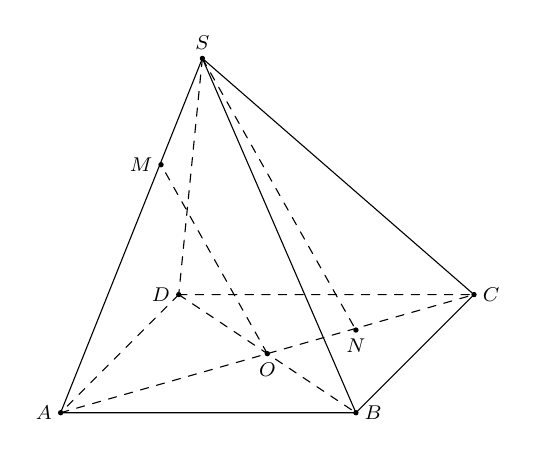
\begin{tikzpicture}[scale=0.75,font=\footnotesize,line join=round,line cap=round,>=stealth]
					 \coordinate (A) at (-4,-2);
					\coordinate (B)  at (1,-2);
					\coordinate (C) at (3,0); 
					\coordinate (D)  at (-2,0);
					\coordinate  (S) at (-1.6,4);
					\coordinate (N) at (1,-0.6); 
					\coordinate (M)  at (-2.3,2.2);
					\coordinate (O) at (intersection of D--B  and A--C);
					\draw[dashed](S)--(D) 
						(D)--(A) 
						(D)--(C) 
						(D)--(B) 
						 (A)--(C)
						 (S)--(N)
						(O)--(M); 
					\draw (S)--(A) 
						(A)--(B) 
						 (S)--(B)
						(S)--(C) 
						(B)--(C); 
					\foreach \i in  {S,A,B,C,D,M,N,O}{\draw[fill=](\i) circle (1pt);}
					\foreach \i in {S}{\draw (\i)  node[scale=0.9,above]{$\i$};}
					\foreach \i in {M,D,A}{\draw (\i)  node[scale=0.9,left]{$\i$};}
					\foreach \i in {O,N}{\draw (\i)  node[scale=0.9,below]{$\i$};}
					\foreach \i in {B,C}{\draw (\i)  node[scale=0.9,right]{$\i$};}
				\end{tikzpicture}
		\end{center}
		\begin{itemchoice}
			\itemch Trong mặt phẳng $(SAC)$ kẻ $SN \parallel OM$ với $N \in AC$. Khi đó $N$ thuộc mặt phẳng $(ABCD)$ nên $N$ là hình chiếu  song song của $S$ lên mặt phẳng $(ABCD)$ theo phương $OM$.
			\itemch Tam giác $SAN$ có $OM \parallel SN \Rightarrow \dfrac{AM}{AS} = \dfrac{AO}{AN} = \dfrac{2}{3}$ (định  lí Thales).\\
			Suy ra $\dfrac{AO}{AN} = \dfrac{2}{3}$, không phải $\dfrac{1}{3}$. 
			\itemch Ta có $\dfrac{AC}{2} : AN  = \dfrac{2}{3} \Rightarrow \dfrac{AC}{AN} = \dfrac{4}{3} \Rightarrow \dfrac{AN}{AC} = \dfrac{3}{4}$.
			\itemch Ta có $\dfrac{CN}{CA} =  \dfrac{1}{4}$.
		\end{itemchoice}
	} 
\end{ex}

% nguồn: Ok_dungsai_lop11_Lan2
\begin{ex}%[1H4V6-2]%[ma:77f4b3a0]
	Cho hình lăng trụ $ABC  . A'B'C'$.
	 \choiceTF
		{\True $AA' \parallel CC'$} 
		{\True $A'$ là hình chiếu của $A$ trên mặt phẳng $\left(A'B'C'\right)$ qua  phép chiếu song song theo phương $CC'$}
		{\True Gọi $M$ là một  điểm trên đoạn thẳng $AB$. Hình chiếu của $M$ trên mặt phẳng $\left(A'B'C'\right)$ qua phép chiếu song song theo phương $BB'$ là điểm $M' \in A'B'$}
		{\True Gọi $O$ là tâm của hình bình hành $BCC'B'$. Ảnh của $O$ qua phép chiếu song song theo  phương $AA'$ trên mặt phẳng $\left(A'B'C'\right)$ là trung điểm của $B'C'$}
	 \loigiai{
		\begin{center}
			\begin{tikzpicture}[scale=0.75,font=\footnotesize,line join=round,line cap=round,>=stealth]
					 \coordinate (B) at (0,0.6);
					\coordinate (A) at  (-2,2);
					\coordinate (C) at (3,2); 
					 \coordinate (A') at (-3,-2);
					\coordinate (B')  at (-1,-3.4);
					 \coordinate (C') at (2,-2);
					\coordinate  (M') at ($(A')!0.5!(B')$);
					 \coordinate (M) at ($(A)!0.5!(B)$);
					\coordinate  (I) at ($(C')!0.5!(B')$);
					\coordinate (O)  at (intersection of B--C' and C--B');
					\draw  (A)--(C)
						 (A)--(B)
						(B)--(C) 
						(A')--(B') 
						(B')--(C') 
						(B)--(C') 
						(C)--(B') 
						(O)--(I) 
						(A)--(A') 
						 (B)--(B')
						(C)--(C') 
						 (M)--(M');
					 \draw[dashed](A')--(C');
					\foreach \i in {A,A'}{\draw (\i)  node[scale=0.9,left]{$\i$};}
					 \foreach \i in {A,B,C,O,I,A',B',C',I,M,M'}{\draw[fill=](\i) circle (1pt);}
					\foreach  \i in {M,B}{\draw (\i) node[scale=0.9,above]{$\i$};}
					\foreach \i in {C,C'}{\draw  (\i) node[scale=0.9,right]{$\i$};}
					\foreach \i in {M',B',I}{\draw (\i) node[scale=0.9,below]{$\i$};} 
					\foreach  \i in {O}{\draw (\i) node[scale=0.9,right]{$\i$};}
				\end{tikzpicture}
		\end{center}
		\begin{itemchoice}
			\itemch Vì  $AA' \parallel CC'$.
			\itemch $A'$ thuộc $(A'B'C')$ nên $A'$  là hình chiếu song song của $A$ trên mặt phẳng $(A'B'C')$ theo phương $CC'$.
			\itemch  Trong mặt phẳng $(ABB'A')$, kẻ đường thẳng $MM' \parallel BB'$ với $M' \in A'B'$. Khi đó $M'$ là hình chiếu song song của $M$ trên mặt phẳng $(A'B'C')$ theo phương $BB'$.
			\itemch Gọi $I$ là trung điểm của $B'C'$. Vì $OI$ là đường trung bình của tam giác $BB'C'$ nên $OI \parallel BB' \Rightarrow OI \parallel AA'$. Mà $I \in (A'B'C')$ nên $I$ là ảnh của $O$  trên mặt phẳng $(A'B'C')$ qua phép chiếu song song theo phương $AA'$.
		\end{itemchoice}
	} 
\end{ex}

% nguồn: Ok_dungsai_lop11_Lan2
\begin{ex}%[1H4V6-2]%[ma:ffce0b6c]
	Cho hình lăng trụ $ABC . A'B'C'$. Điểm $I$ và $I'$ lần lượt là trung điểm của đoạn thẳng $AB$ và  $A'B'$.
	 \choiceTF
		{\True $AI' \parallel  IB'$}
		{ Hình chiếu song song của $I$ trên mặt phẳng $\left(A'B'C'\right)$ phương $A'I$ là  điểm $C'$}
		{\True Trong mặt phẳng $(A'B'C')$ vẽ hình  bình hành $A'C'MI'$, suy ra $ACMI'$ là hình bình hành}
		{\True $M$ là hình chiếu  song song của $C$ theo phương $AI'$ trên mặt phẳng $\left(A'B'C'\right)$}
	\loigiai{ 
		\begin{center}
			\begin{tikzpicture}[scale=0.75,font=\footnotesize,line join=round,line cap=round,>=stealth]
					\coordinate (A)  at (-2,3);
					 \coordinate (B) at (3,3);
					\coordinate (C) at (0,1.6); 
					 \coordinate (A') at (-2.6,-2);
					\coordinate (B') at (2.4,-2); 
					\coordinate  (C') at (-0.5,-3.4);
					\coordinate  (I) at ($(A)!0.5!(B)$);
					\coordinate (I') at ($(A')!0.5!(B')$); 
					\coordinate (M) at (2,-3.4); 
					\draw[dashed](A')--(B') 
						 (A)--(I')
						(I)--(B') 
						(I')--(M) 
						(B')--(C'); 
					\draw (A)--(B) 
						 (A)--(C)
						 (C)--(B)
						(A')--(C') 
						(C')--(M) 
						(C)--(C') 
						 (A)--(A')
						 (B)--(B')
						(C)--(M); 
					\foreach \i  in {A,B,C,A',B',C',I,I',M}{\draw[fill=](\i) circle (1pt);}
					\foreach \i in {A,I,B}{\draw  (\i) node[scale=0.9,above]{$\i$};}
					\foreach \i in  {A'}{\draw (\i) node[scale=0.9,left]{$\i$};}
					\foreach \i  in {B',M}{\draw (\i) node[scale=0.9,right]{$\i$};}
					\foreach  \i in {I'}{\draw (\i) node[scale=0.9,above right]{$\i$};}
					 \node[scale=0.9,anchor=north east] at (C) {$C$};
					\node[scale=0.9,anchor=north east] at (C')  {$C'$};
				\end{tikzpicture}
		\end{center}
		\begin{itemchoice}
			\itemch Ta có $\heva{&AI \parallel  B'I'\\
			&AI = B'I' =  \dfrac{AB}{2}}$\\
			$\Rightarrow AIB'I'$ là hình bình hành.\\ 
			Suy  ra $AI' \parallel IB'$.
			\itemch Hình chiếu song song của $I$ trên mặt phẳng $(A'B'C')$ theo phương $A'I$ là  điểm $B'$, không phải $C'$.
			\itemch  Trong mặt phẳng $(A'B'C')$ vẽ hình bình hành $A'C'MI'$. Ta có $MI' \parallel A'C'$ và $MI'=A'C'$, đồng thời $A'C' \parallel AC$, nên suy ra $MI' \parallel AC$ và $MI'=AC$. Do đó $ACMI'$ là hình bình hành.
			\itemch Vì $AI' \parallel CM$ và  $M \in (A'B'C')$ nên $M$ chính là hình chiếu song song của $C$ theo phương $AI'$ trên mặt phẳng $(A'B'C')$.
		\end{itemchoice}
	 }
\end{ex}


%%%%%%%%%%%%%%%% TRẢ LỜI NGẮN %%%%%%%%%%%%%%%%

% nguồn: Ok_TraLoiNgan_Lop11_Lan1
\begin{ex}%[1H4H6-2]%[ma:0a1669d2]
	Cho hình chóp $S.ABC$  có $ABC$ và $SAB$ là các tam giác đều cạnh $a$, mặt bên $\left(SAB\right)$ vuông góc với đáy. Gọi $\alpha$ là góc phẳng nhị diện $\left[S,BC,A\right]$. Tính giá trị $\cos\alpha$ (kết quả làm tròn đến hàng phần trăm).
	 \shortans{0,45}
	\loigiai{ 
	 \immini{
		 Gọi $H$ là trung điểm của $AB$.\\
		Do tam giác $SAB$  đều nên $SH\perp AB$.\\
		Ta có 
		 $\heva{
		&\left(SAB\right) \perp \left(ABC\right)\\ 
		&\left(SAB\right)  \cap \left(ABC\right)\\
		&SH\perp AB 
		} 
		 \Rightarrow SH\perp \left(ABC\right)$.\\
		Gọi $M$ là trung điểm của $BC$.\\ 
		Do tam giác $ABC$ đều nên $AM\perp  BC$.\\
		Gọi $I$  là trung điểm của $BM$.\\
		Ta có $HI$ là đường trung bình của tam giác  $ABM$.\\
		Suy ra $HI\parallel AM\Rightarrow HI\perp  BC$.\\
		Mà $SH \perp AB$ nên $BC\perp  \left(SHI\right)$.\\
		 Suy ra $BC\perp SI$.\\
		} 
		 {
		\begin{tikzpicture}[scale=0.8,font=\footnotesize,line join=round,line cap=round,>=stealth]
				\coordinate  (A) at (-2,0);
				 \coordinate (C) at (3,0);
				 \coordinate (B) at (0,-2);
				\coordinate (H) at ($(A)!0.5!(B)$); 
				 \coordinate (S) at ($(H)+(0,5)$);
				\coordinate (M) at ($(B)!0.5!(C)$); 
				\coordinate (I) at  ($(B)!0.5!(M)$);
				\foreach \i  in {A,B,C,H,I}{\draw (S)--(\i);}
				\draw (A)--(B)--(C); 
				\draw[dashed,thin](A)--(C) 
					(A)--(M) 
					 (A)--(I)--(H);
				\pic[draw,thin,angle radius=2mm] {right angle  = C--M--A}
					pic[draw,thin,angle radius=2mm] {right  angle = B--H--S}
					pic[draw,thin,angle radius=2mm] {right angle =  H--I--B}
					pic[draw,thin,angle radius=2mm] {right  angle = S--I--C}
					pic[draw,thin,angle radius=4mm]  {angle = S--I--H};
				\foreach  \i/\g in {A/-120,B/-90,C/-90,S/90,H/-120,M/-60,I/-60}{\draw[fill=black](\i) circle (1pt)
					($(\i)+(\g:4mm)$)  node[scale=1]{$\i$};}
			\end{tikzpicture}
		 }
		 \noindent
		Ta có $HI\perp BC$ và $SI\perp BC$ suy ra $\widehat{SIH}$ là  góc phẳng nhị diện $\left[S,BC,A\right]$.\\
		Xét tam giác $SAB$ đều cạnh $a$ suy ra $SH=\dfrac{a\sqrt{3}}{2}$.\\ 
		Xét tam giác $ABC$  đều cạnh $a$ suy ra $AM=\dfrac{a\sqrt{3}}{2}$ và $HI=\dfrac{1}{2}AM=\dfrac{a\sqrt{3}}{4}$.\\
		Xét tam giác $SHI$ vuông tại $H$  suy ra $SI=\sqrt{SH^2+HI^2}=\dfrac{\sqrt{15} a}{4}$.\\
		Xét tam giác $SHI$ vuông tại $H$ suy ra  $\cos\alpha=\cos \widehat{SIH}=\dfrac{HI}{SI}=\dfrac{\sqrt{5}}{5} \approx 0{,}45$.
	 }
\end{ex}

% nguồn: Ok_TraLoiNgan_Lop11_Lan1
\begin{ex}%[1H4V6-2]%[ma:2141de24]
	Cho hình chóp $S.ABCD$ đáy là hình bình hành, $O$ là tâm của đáy. Trên cạnh $SB$, $SD$ lần lượt lấy điểm $M$, $N$ sao cho $SM=2MB$  và $SN=\dfrac{1}{3}SD$. Hình chiếu của $M$, $N$ qua phép chiếu song song lên mặt phẳng $(ABCD)$ theo phương $SO$ lần lượt là $P$, $Q$. Tính tỉ số $\dfrac{OP}{OQ}$.
	\shortans{2} 
	 \loigiai{
	\immini 
		{ 
		Do $P$ là hình chiếu song song của $M$ lên mặt phẳng $(ABCD)$ theo phương $SO$ nên $SM  \parallel SO$.\\
		Áp dụng định lí Thales ta có $\dfrac{BM}{BS}=\dfrac{BP}{BO}$.\\ 
		Mà  $SM=2MB$ nên $\dfrac{BP}{BO}=\dfrac{1}{3}$ suy ra $\dfrac{OP}{OB}=\dfrac{2}{3}$. (1)\\
		Chứng minh tương  tự ta có $\dfrac{OQ}{OD}=\dfrac{1}{3}$. (2)\\
		Do $ABCD$ là hình bình hành tâm $O$ nên $BO=OD$.  (3)\\
		Từ (1), (2) và  (3) ta có $\dfrac{OP}{OQ}=2$.
		} 
		 {
		\begin{tikzpicture}[line join=round,line cap=round]
				 \path
					(0,0)  coordinate (B)
					 (3,0) coordinate (C)
					(5,1.5)  coordinate (D)
					 (2,1.5) coordinate (A)
					 (2.5,4) coordinate (S)
					($(S)!1/3!(D)$) coordinate (N) 
					($(S)!2/3!(B)$)  coordinate (M)
					 ($(A)!1/2!(C)$) coordinate (O)
					 ($(B)!1/3!(O)$) coordinate (P)
					($(D)!2/3!(O)$) coordinate (Q); 
				\draw (S)--(B)--(C)--(D)--cycle  (S)--(C);
				\draw[dashed,thin] (B)--(A)--(D) 
					(S)--(A)--(C) 
					(M)--(P) 
					 (N)--(Q)
					(S)--(O) 
					 (B)--(D);
				\foreach \i/\g in {A/135,B/180,C/-45,D/0,S/90,N/45,M/180,P/-45,O/-90,Q/-90}{\draw[fill=black](\i)  circle (1pt)
					($(\i)+(\g:3mm)$) node[scale=1]{$\i$};} 
			\end{tikzpicture}
		 }
	} 
\end{ex}


%%%%%%%%%%%%%%%% TỰ LUẬN %%%%%%%%%%%%%%%%

% nguồn: Ok_TuanLuan_Toan11_Lan2
\begin{ex}%[1H4N6-2]%[ma:856f0d53]
	Cho hình hộp $ABCD.A'B'C'D'$. Xác định ảnh của các điểm $A'$, $B'$, $C'$, $D'$ qua phép chiếu  song song lên mặt phẳng $(ABCD)$ theo phương $A'A$.
	\begin{center}
		\begin{tikzpicture}[scale=1,font=\footnotesize,line join=round,line cap=round,>=stealth]
				 \path (-1,1.7) coordinate (h)
					 (0,0) coordinate (B)
					(3,0)  coordinate (C)
					(3.8,1) coordinate (D) 
					 ($(B)+(D)-(C)$) coordinate (A);
				\foreach \p in {A,B,C,D}\path ($(\p)+(h)$) coordinate  (\p');
				 \draw (A')--(B')--(B)--(C)--(D)--(D')--cycle (B')--(C')--(D')
					 (C)--(C');
				 \draw[dashed] (B)--(A)--(D)
					(A)--(A'); 
				\foreach  \p/\g in {A/180,B/240,C/-60,D/0,A'/90,B'/180,C'/120,D'/45} \fill (\p) circle (1pt)+(\g:0.3) node{$\p$};
			\end{tikzpicture}
	\end{center}
	 \loigiai{
		Vì $ABCD.A'B'C'D'$ là hình hộp nên các cạnh $AA', BB', CC',  DD'$ song song với nhau.\\
		Do đó các điểm $A$, $B$, $C$, $D$ lần lượt là ảnh của  $A'$, $B'$, $C'$, $D'$ qua phép chiếu song song lên mặt phẳng $(ABCD)$ theo phương $A'A$.
	 }
\end{ex}

% nguồn: Ok_TuanLuan_Toan11_Lan2
\begin{ex}%[1H4N6-2]%[ma:08ae5bbf]
	Cho mặt phẳng $(P)$ có đoạn thẳng $A B$  và đường thẳng $\ell$ cắt mặt phẳng $(P)$. Giả sử đường thẳng $A B$ không song song với $\ell$. Nêu cách xác định hình chiếu song song của đoạn thẳng $A B$ trên mặt phẳng $(P)$ theo phương $\ell$.
	\begin{center}
		\begin{tikzpicture}[scale=1,font=\footnotesize,line join=round,line cap=round,>=stealth]
				 \def \a{80};
				\def \b{10}; 
				\path (0,0)  coordinate (V)
					(4,0) coordinate  (X)
					(5.5,1.5) coordinate (Y) 
					 ($(V)+(Y)-(X)$) coordinate (Z)
					(5.5,0.5) coordinate  (L)
					($(L)+(\a:1.8)$) coordinate (L') 
					(1.9,0.7) coordinate (A')--++(1.7,0) coordinate  (B')--++(\a:1.5) coordinate (B)--++(\b:1) coordinate (b)
					 (A')--++(\a:1) coordinate (a)
					(intersection of A'--a and  B--b) coordinate (A)
					(intersection of Y--Z and  A--A') coordinate (z)
					(intersection of Y--Z  and B--B') coordinate (y);
				\fill[gray!20] (V)--(X)--(Y)--(Z)--cycle; 
				\draw (L)--($(L)!1.1!(L')$)  node[right]{$\ell$}
					(A)--(B)--(B')--(A')--cycle  (y)--(Y)--(X)--(V)--(Z)--(z);
				 \draw[dashed] (y)--(z);
				\foreach  \p/\g in {A/90,A'/-90,B'/-90,B/90} \fill (\p) circle (1pt)+(\g:0.3) node{$\p$};
				\draw  pic[draw,"$P$",angle eccentricity=0.7,angle radius=0.8cm]{angle=X--V--Z};
			\end{tikzpicture}
	\end{center}
	 \loigiai{
		Gọi $A', B'$ lần lượt là hình chiếu song song của $A$, $B$ trên mặt phẳng $(P)$ theo phương  $\ell$.\\
		Khi đó, hình chiếu song song của đoạn thẳng $AB$ trên mặt phẳng $(P)$ theo phương  $\ell$ là đoạn thẳng $A'B'$.
	 }
\end{ex}

% nguồn: Ok_TuanLuan_Toan11_Lan2
\begin{ex}%[1H4H6-2]%[ma:5c16d115]
	Nếu tam giác $A'B'C'$ là hình chiếu của tam giác $ABC$ qua một phép chiếu song song thì tam giác $ABC$ có phải là hình chiếu của tam giác $A'B'C'$ qua một phép chiếu song song hay không? Hãy  giải thích.
	\loigiai{ 
		\begin{center}
			\begin{tikzpicture}[scale=1,font=\footnotesize,line join=round,line cap=round,>=stealth]
					 \path
						 (0,0) coordinate (A)
						(4,0) coordinate  (C)
						 (2.5,-1) coordinate (B)
						 (-0.5,-3) coordinate (x)
						($(A)+(x)$) coordinate  (A')
						($(B)+(x)$)  coordinate (B')
						($(C)+(x)$)  coordinate (C');
					\draw 
						(A)--(B)--(C)--cycle 
						 (A)--(A')
						(B)--(B') 
						(C)--(C') 
						 (A')--(B')--(C');
					\draw[dashed] (C')--(A'); 
					\foreach \x/\g in {A/60,B/120,C/90,A'/-75,C'/-90,B'/-120} \fill(\x) circle  (1pt)+(\g:0.3) node{$\x$};
				\end{tikzpicture}
		\end{center}
		Theo giả thiết, tam giác $A'B'C'$ là hình chiếu của tam giác $ABC$ qua  phép chiếu song song theo phương của đường thẳng $AA'$ lên mặt phẳng $(A'B'C')$.\\
		Chú  ý rằng $AA' \parallel BB' \parallel CC'$.\\
	Khi đó ta có thể coi tam giác $ABC$ là hình chiếu của tam giác $A'B'C'$ qua phép chiếu song song theo phương của đường thẳng $AA'$ lên  mặt phẳng $(ABC)$.}
\end{ex}

% nguồn: Ok_TuanLuan_Toan11_Lan2
\begin{ex}%[1H4H6-2]%[ma:a7b8380e]
	Cho mặt phẳng $(P)$, tam giác $ABC$ và đường thẳng $\ell$ cắt mặt phẳng $(P)$ sao cho các đường thẳng $AB$, $BC$, $CA$ đều không song song hoặc trùng với đường thẳng $\ell$. Xác định hình chiếu song song của tam giác $ABC$ trên mặt phẳng $(P)$ theo phương $\ell$ trong mỗi trường hợp sau 
	\begin{enumerate}
		\item Mặt phẳng $(ABC)$ không song  song với $\ell$.
		\item Mặt phẳng ($ABC$) song  song hoặc chứa $\ell$.
	\end{enumerate}
	\loigiai{ 
		\begin{center}
			\begin{tikzpicture}[scale=1,font=\footnotesize,line join=round,line cap=round,>=stealth]
					\begin{scope}
						 \def \a{80};
						\def  \b{-10};
						\path  (0,0) coordinate (V)
						(4,0)  coordinate (X)
						(5.5,1.5) coordinate  (Y)
						($(V)+(Y)-(X)$)  coordinate (Z)
						(0.1,0.9) coordinate  (L)
						($(L)+(\a:1.8)$) coordinate (L') 
						(1.7,1.2) coordinate (A')--++(2.5,0) coordinate (C')--++(-1,-0.7)  coordinate (B')--++(\a:1.3) coordinate (B)
						(A')--++(\a:1.5) coordinate  (A)
						 (C')--++(\a:1.7) coordinate (C)
						(intersection of Y--Z and A--A') coordinate (z) 
						(intersection of Y--Z and C--C') coordinate (y); 
						\fill[gray!20] (V)--(X)--(Y)--(Z)--cycle; 
						 \draw[dashed](y)--(z)
						 (A')--(C');
						\draw (L)--($(L)!1.1!(L')$)  node[right]{$\ell$}
						(A)--(A') 
						(B)--(B') 
						(C)--(C') 
						(y)--(Y)--(X)--(V)--(Z)--(z) 
						(A)--(B)--(C)--cycle (A')--(B')--(C'); 
						\foreach \p/\g in {A'/-90,A/90,B/0,C/90,B'/-90,C'/-90} \fill (\p) circle (1pt)+(\g:0.3)  node{$\p$};
						\draw pic[draw,"$P$",angle eccentricity=0.7,angle radius=0.8cm]{angle=X--V--Z}; 
						\draw  ($(V)!0.6!(X)-(0,0.6)$) node[]{a)};
					\end{scope}
					\begin{scope}[xshift=7cm]
						\def \a{80}; 
						 \def \b{-10};
						 \path (0,0) coordinate (V)
						(4,0) coordinate  (X)
						 (5.5,1.5) coordinate (Y)
						($(V)+(Y)-(X)$) coordinate (Z) 
						(0.1,0.9)  coordinate (L)
						($(L)+(\a:1.8)$) coordinate  (L')
						(1.7,0.7) coordinate (A')--++(2.5,0) coordinate (C')--++(-1.5,0) coordinate (B')--++(\a:1.2)  coordinate (B)
						(A')--++(\a:1.9) coordinate  (A)
						 (C')--++(\a:1.7) coordinate (C)
						(intersection of Y--Z and  A--A') coordinate (z)
						 (intersection of Y--Z and C--C') coordinate (y);
						 \fill[gray!20] (V)--(X)--(Y)--(Z)--cycle;
						\draw[dashed](y)--(z) 
						 (A')--(C');
						 \draw (L)--($(L)!1.1!(L')$) node[right]{$\ell$}
						 (A)--(A')
						(B)--(B') 
						(C)--(C') 
						 (y)--(Y)--(X)--(V)--(Z)--(z)
						(A)--(B)--(C)--cycle (A')--(B')--(C'); 
						\foreach \p/\g in  {A'/-90,A/90,B/-30,C/90,B'/-90,C'/-90} \fill (\p) circle (1pt)+(\g:0.3) node{$\p$};
						\draw pic[draw,"$P$",angle eccentricity=0.7,angle  radius=0.8cm]{angle=X--V--Z};
						\draw  ($(V)!0.6!(X)-(0,0.6)$) node[]{b)};
					\end{scope}
				\end{tikzpicture}
		\end{center}
		Gọi $A'$,  $B'$, $C'$ lần lượt là hình chiếu song song của ba điểm $A$, $B$, $C$ trên mặt phẳng $(P)$ theo phương $\ell$.
		\begin{enumerate}
			\item Hình chiếu của tam giác $ABC$ trên mặt phẳng $(P)$ là tam giác $A'B'C'$ (Hình a). 
			\item Ba điểm $A'$, $B'$, $C'$ thuộc giao tuyến của hai mặt phẳng $(ABC)$ và $(P)$ nên ba điểm $A'$, $B'$, $C'$ thẳng hàng và có một điểm nằm giữa hai  điểm còn lại. Giả sử điểm $B'$ nằm giữa hai điểm $A'$ và $C'$. Khi đó, hình chiếu song song của tam giác $ABC$ trên mặt phẳng $(P)$ là đoạn thẳng $A'C'$ (Hình b).
		\end{enumerate}
	} 
\end{ex}
